\documentclass[12pt,a4paper]{article}
\usepackage{graphicx}
\usepackage{amsmath}

\begin{document}

\begin{enumerate}
    \item Nov. 22. Saturday from 11 AM - 2 PM.
    \item Exam Duration: 1 hour and 30 minutes max., onsite
    \item Type of exam: Multiple Choice, True / False, Problem Solving (answered by coding)
    \item Coverage: 07 Neural networks, RNNs, and Transformers - 12 Social Network Analysis

\end{enumerate}

\section{Neural Network Unit}

Takes weighted sum of inputs, plus a bias.

\[ z = b + w_i x_i\]
\[ z = w \times x + b \]

Instead of just usning z, we'll apply a non linear activation function f:

\[ y = a = f(z) \]
\[ y = a = z = w \times x + b \]

\subsection{Non-linear activation functions}

\textbf{Sigmoid:}
For logistic regression, we use sigmoid:
\[ y = s(z) = 1 / (1 + e^{-z}) \]

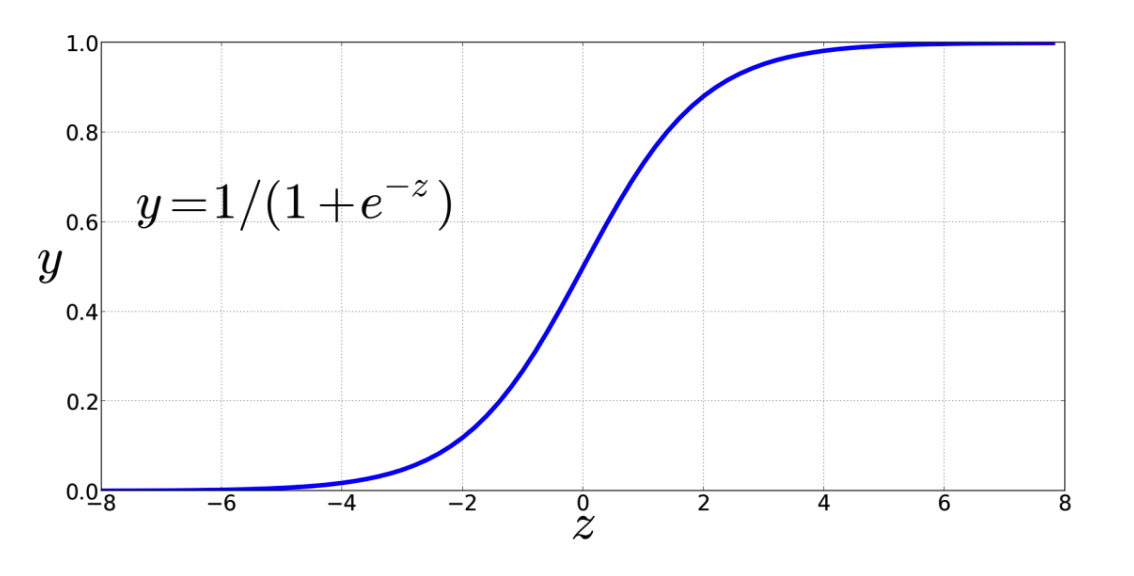
\includegraphics[width=0.5\textwidth]{figures/Sigmoid.png}

\textbf{Final function the unit is computing}

\[ y = s(w \times x + b) = 1 / 1 + e^{-(w \times x + b)} \]

\textbf{Non Linear Activation Functions besides Sigmoid:}

\begin{itemize}
    \item Sigmoid : S shaped curve, output between 0 and 1
    \item Tanh  : Similar to sigmoid, output between -1 and 1
    \item ReLU : max(0, x); avoids vaniishing gradient for large x.
\end{itemize}

\subsection{Perceptrons}

\begin{itemize}
    \item Simple neural unit.
    \item Binary output, 0 or 1.
    \item No non-linear activation function
\end{itemize}

\[
y =
\begin{cases}
0, & \text{if } w \cdot x + b \le 0, \\[6pt]
1, & \text{if } w \cdot x + b > 0.
\end{cases}
\]

\subsection{The XOR problem}

\textit{Can the XOR problem be calculated using a single perceptron?}

\begin{tabular}
{|c|c|c|}
\hline
X1 & X2 & Y \\
\hline
0 & 0 & 0 \\
0 & 1 & 1 \\
1 & 0 & 1 \\
1 & 1 & 0 \\
\hline
\end{tabular}

\textbf{Solution:} No, because the data is not linearly separable. XOR can be calculated by a layered network of units.


\subsection{Feedforward Neural Networks}
\begin{itemize}
    \item Can also be called \textbf{multi-layer perceptrons} (or MLPs) for historial reasons
\end{itemize}

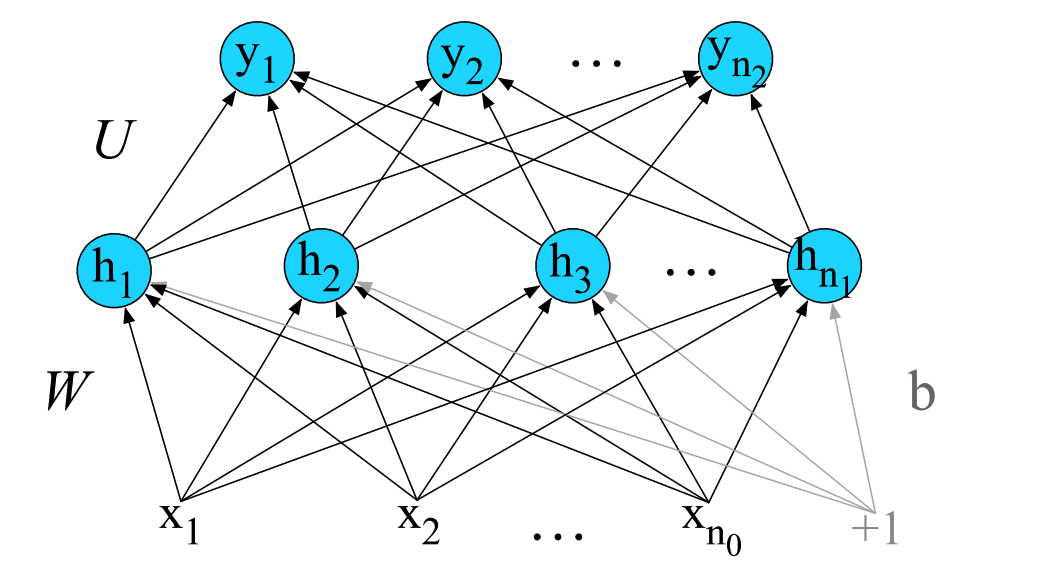
\includegraphics[width=0.5\textwidth]{figures/FeedforwardNN.png}

\subsection{Binary Logistic Regression as a 1-layer neural network}

(we don't count the input layer in counting layers!)

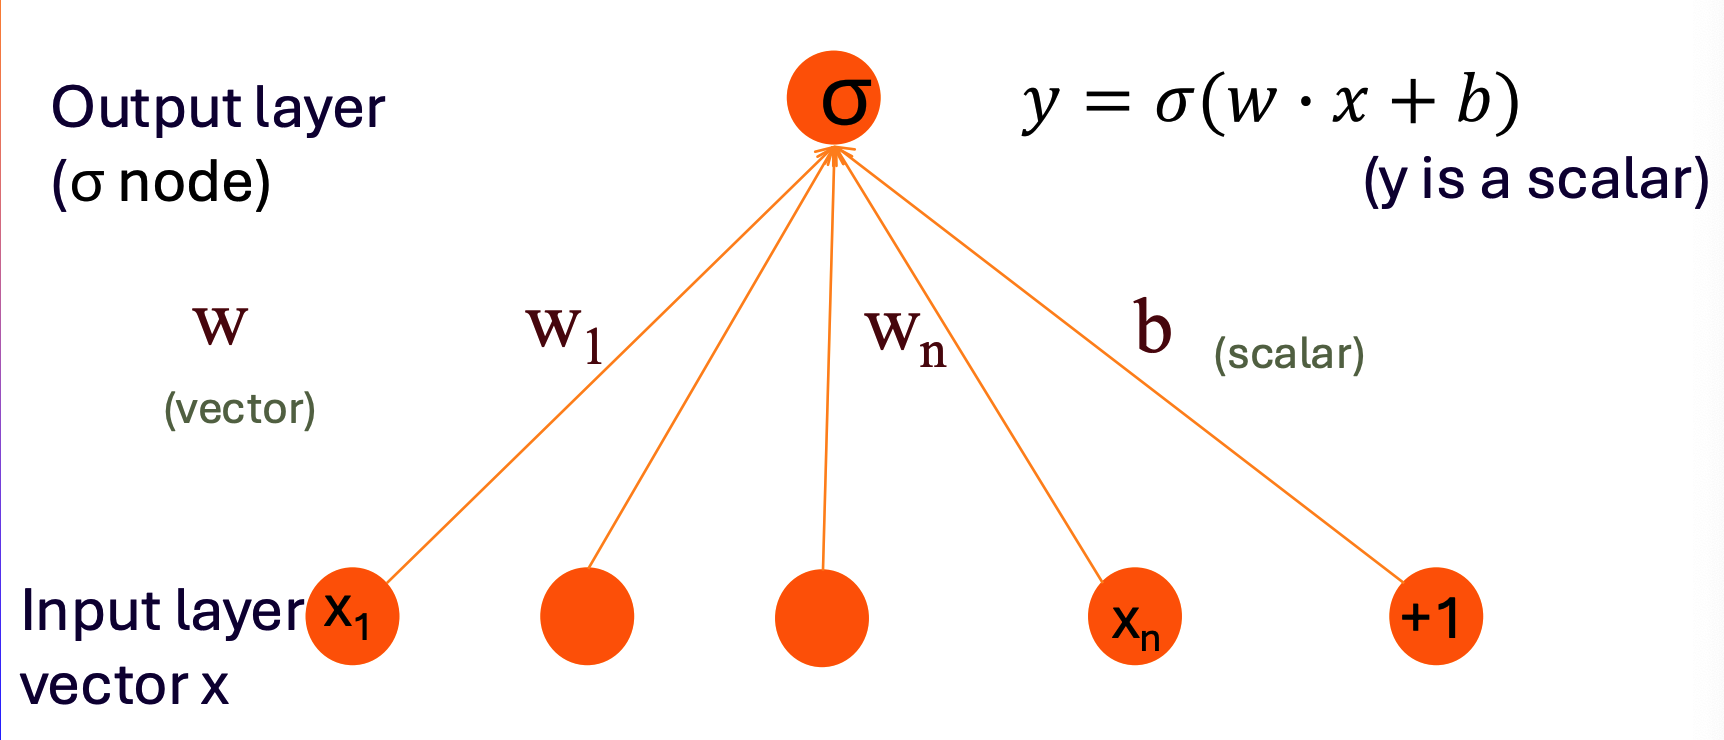
\includegraphics[width=0.5\textwidth]{figures/BinaryLogRegOneLayer.png}

\subsection{Multinomial Logistic Regression as a 1-layer neural network}

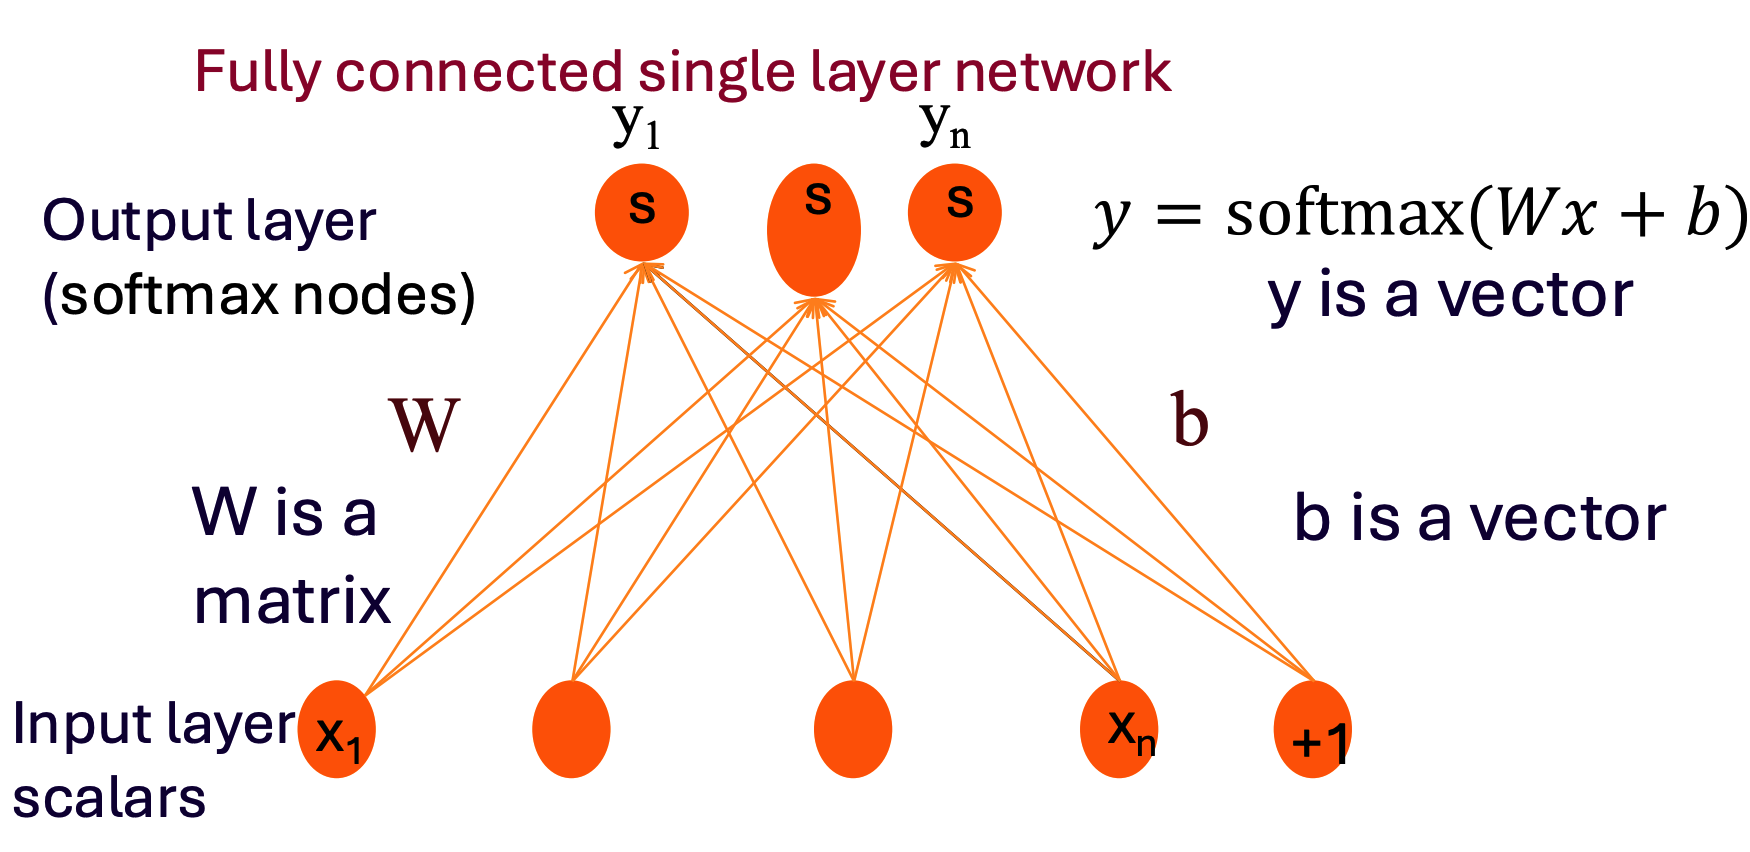
\includegraphics[width=0.5\textwidth]{figures/MultinomialLogisticRegression.png}

\end{document}